\subsection{Motivation}

First introduced by Ying et. al \cite{Ying:2004:JCP}, the kernel-independent FMM (\textbf{\gls{KIFMM}})
provides an algorithm that maintains the basic recursive structure and $O(N)$
asymptotic complexity of the analytic FMM, but without the requirement for the
implementation of analytic expansions of the kernel function for each kernel.
Instead the method relies only on kernel function evaluations. This allows
software implementations to be written in an easily extensible manner for different
kernels. The main difference to the analytic FMM of Section \ref{sec:1_1_fmm_overview},
lies in the the way that source and target densities are represented, and how
the \gls{M2M}, \gls{L2L} and \gls{M2L} operators are computed.

\subsection{Algorithm Structure \& Analysis}

For the \gls{KIFMM} presented in \cite{Ying:2004:JCP} the \gls{far-field}, $\mathcal{F}^B$, and
\gls{near-field}, $\mathcal{N}^B$, have precise specifications. For a given box $B$
centered at $\mathbf{c}$ with sides of length 2$r$, $\mathcal{N}^B$ is a box
centered at $\mathbf{c}$ with sides of length 6$r$. The \gls{far-field} is then
defined as $\mathbb{R}^d / \mathcal{N}^B$, where $d$ is spatial dimension.
Here, $B$ is in the \gls{near-field}. Consider the potential in the \gls{far-field} $\mathcal{F}^B$, generated by a
set of \gls{source-particles}, described by \textbf{\gls{source-densities}}
$\{\phi_i, \> i \in I^B_s \}$ where $I^B_s$ is the set of indices for the \gls{source-particles}
in box $B$\footnote{This notation matches that used in \cite{Ying:2004:JCP}
in order for ease of reference.}. Specifying the indices for the \gls{source-particles}
specifically to make it clear that they may be distinct from the \gls{target-particles}.
These \gls{source-particles} can be equivalently described with an \textbf{upward \gls{equivalent-density}}
distribution $\phi^{B,u}$ supported at discrete points on an \textbf{upward \gls{equivalent-surface}}
$\mathbf{y}^{B, u}$ that encloses the set of source particles. The KIFMM relies
on the assumption that the potential produced by the equivalent densities is smooth,
which is guaranteed in the case that $\mathbf{y}^{B,u}$ does not overlap with the
far-field $\mathcal{F}^B$ \cite{Ying:2004:JCP}, furthermore the requirement that
$\mathbf{y}^{B,u}$ must enclose all particles in $B$ leads to the requirement
that it must also not overlap with $B$. For second-order linear elliptic
\textbf{\gls{PDE}}s, for which the KIFMM is defined,
and of which equation (\ref{eq:poisson}) is an example, the solution for the
potential in the far field, which can be seen as an exterior Dirichlet problem,
is guaranteed to be unique \cite{Ying:2004:JCP}. Therefore, the potentials
induced by the source particles and the equivalent densities satisfy are
guaranteed to be equivalent in the far field $\mathcal{F}^B$ if they coincide
at the boundary of the far field $\mathcal{F}^B$, or anywhere between the boundary
of the far field and the upward \gls{equivalent-surface}. This boundary is referred to
as the \textbf{upward \gls{check-surface}}, $\mathbf{x}^{B, u}$, and the entire
scheme is illustrated in figure (\ref{fig:1_2_upward_downward_surfaces}A).
The equality of the potentials from the source points and the equivalent density
can be stated mathematically as follows,

\begin{equation}
\int_{\mathbf{y}^{B,u}} K(\mathbf{x}, \mathbf{y})\phi^{B, u} d\mathbf{y} = \sum_{i \in I_s^B} K(\mathbf{x}, \mathbf{y})\phi_i = q^{B, u} \> \> \text{for any} \> \> \mathbf{x} \in \mathbf{x}^{B, u}
\label{eq:1_2_p2m}
\end{equation}

\begin{figure}[!h]
    \centering
    {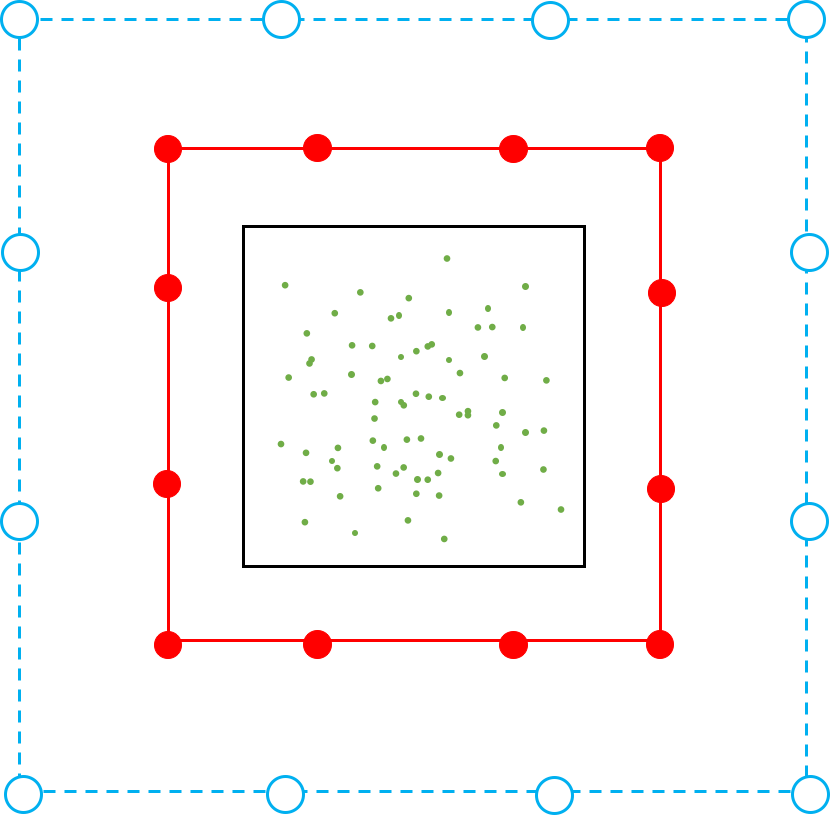
\includegraphics[width=0.3\textwidth]{introduction/upward_surface.png}}
    \hfill
  {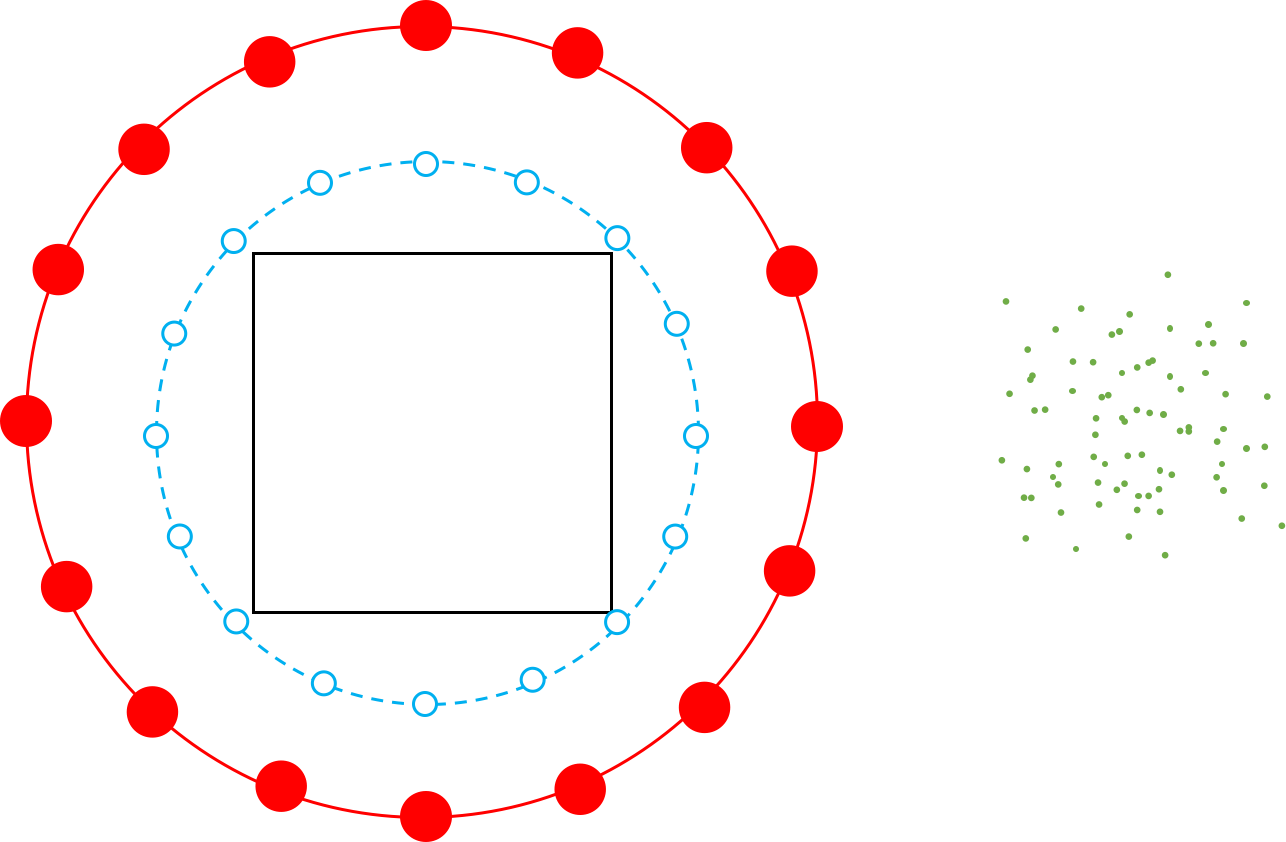
\includegraphics[width=0.4\textwidth]{introduction/downward_surface.png}}
  \vspace{0pt}
  \caption{Cross section of three dimensional cubic upward/downward equivalent and
    check surfaces. Source points are denoted by green circles. Red solid lines
    denote equivalent surfaces, and blue checked lines denote check surfaces.
    The black solid line defines the box $B$. This figure is adapted directly from \cite{Ying:2004:JCP}.}
  \label{fig:1_2_upward_downward_surfaces}
\end{figure}

where the integral form of (\ref{eq:n_body_problem}) is used for the summation of
the contribution from the equivalent densities, and $q^{B, u}$ is referred to as
the \textbf{upward \gls{check-potential}}, with the other symbols taking their previous
definitions. One can define a very similar scheme for the case in which the source
densities are in $\mathcal{F}^B$, as a potential induced by a
\textbf{downward \gls{equivalent-density}} $\phi^{B,d}$ supported at discrete points
on a \textbf{downward \gls{equivalent-surface}} $\mathbf{y}^{B,d}$. This surface
needs to be located between the boundary of $\mathcal{F}^B$ and $B$, and again
as the solution for interior Dirichlet style problems for the types of PDEs
considered in this thesis is also unique \cite{Ying:2004:JCP}, one can equate the potentials generated
by the source points with that generated by the equivalent densities at some surface
between $\mathbf{y}^{B,d}$ and $B$. This surface is called the \textbf{downward \gls{check-surface}},
$\mathbf{x}^{B,d}$, and a corresponding mathematical statement of the equality of
the potentials can be written as follows,

\begin{equation}
    \int_{\mathbf{y}^{B,d}} K(\mathbf{x}, \mathbf{y})\phi^{B, d} d\mathbf{y} = \sum_{i \in I_s^{\mathcal{F}^B}} K(\mathbf{x}, \mathbf{y})\phi_i = q^{B, d} \> \> \text{for any} \> \> \mathbf{x} \in \mathbf{x}^{B, d}
    \label{eq:1_2_p2l}
\end{equation}

where $I_s^{\mathcal{F}^B}$ represents the indices of source points in the \gls{far-field}
of $B$, and $q^{B, d}$ is the \textbf{downward \gls{check-potential}}.

The equation (\ref{eq:1_2_p2m}) is an Fredholm integral
equation, of the first kind, and it's clear that its solution $\phi^{B, u}$
can be seen to be equivalent to the multipole expansion for the \gls{source-particles} contained in $B$. Therefore,
(\ref{eq:1_2_p2m}) can be seen to be correspond to the \gls{P2M}
operation. Similarly, the solution of (\ref{eq:1_2_p2l}) can be seen
to correspond to a particle-to-local, or P2L operation. Crucially, this method of solving
a set of linear equations to find equivalents of the multipole and local expansions
does not depend on finding a series expansion of a kernel function, and just on its evaluation.

Using this language of equivalent densities and check surfaces, one is also able to
write operations equivalent to the \gls{M2M}, \gls{L2L} and \gls{M2L} operations. For a box $A$
and it's parent box $B$, the \gls{M2M} operation can be written as,

\begin{equation}
    \int_{\mathbf{y}^{A,u}} K(\mathbf{x}, \mathbf{y})\phi^{A, u} d\mathbf{y} =   \int_{\mathbf{y}^{B,u}} K(\mathbf{x}, \mathbf{y})\phi^{B, u} d\mathbf{y}, \> \> \text{for any} \> \> \mathbf{x} \in \mathbf{x}^{B, u}
    \label{eq:1_2_m2m}
\end{equation}

Once $\phi^{A, u}$ has been calculated for boxes at the leaf level of the tree,
one can apply (\ref{eq:1_2_m2m}) to evaluate the multipole expansions for all
the boxes containing \gls{source-particles} in the tree in a manner equivalent
to the upward pass of Section \ref{sec:1_1_fmm_overview}. The \gls{M2M} operation is
illustrated in figure (\ref{fig:1_2_m2m_l2l}A).

For the downward pass, the \gls{M2L} operation, between a box $B$ and a box $A$ in its
interaction list can be written as,

\begin{equation}
    \int_{\mathbf{y}^{A,u}} K(\mathbf{x}, \mathbf{y})\phi^{A, u} d\mathbf{y} =   \int_{\mathbf{y}^{B,d}} K(\mathbf{x}, \mathbf{y})\phi^{B, d} d\mathbf{y}, \> \> \text{for any} \> \> \mathbf{x} \in \mathbf{x}^{B, d}
\label{eq:1_2_m2l}
\end{equation}

This is illustrated in figure (\ref{fig:1_2_m2l}). Once the local expansions
have  been computed starting at level 2 of the tree, one can perform the L2L
operation to transfer the local expansion of a parent box to its children,
for a box $A$ and it's child $B$, which can be written as,

\begin{equation}
    \int_{\mathbf{y}^{A,d}} K(\mathbf{x}, \mathbf{y})\phi^{A, d} d\mathbf{y} =   \int_{\mathbf{y}^{B,d}} K(\mathbf{x}, \mathbf{y})\phi^{B, d} d\mathbf{y}, \> \> \text{for any} \> \> \mathbf{x} \in \mathbf{x}^{B, d}
    \label{eq:1_2_l2l}
\end{equation}

\begin{figure}[!h]
    \centering
    {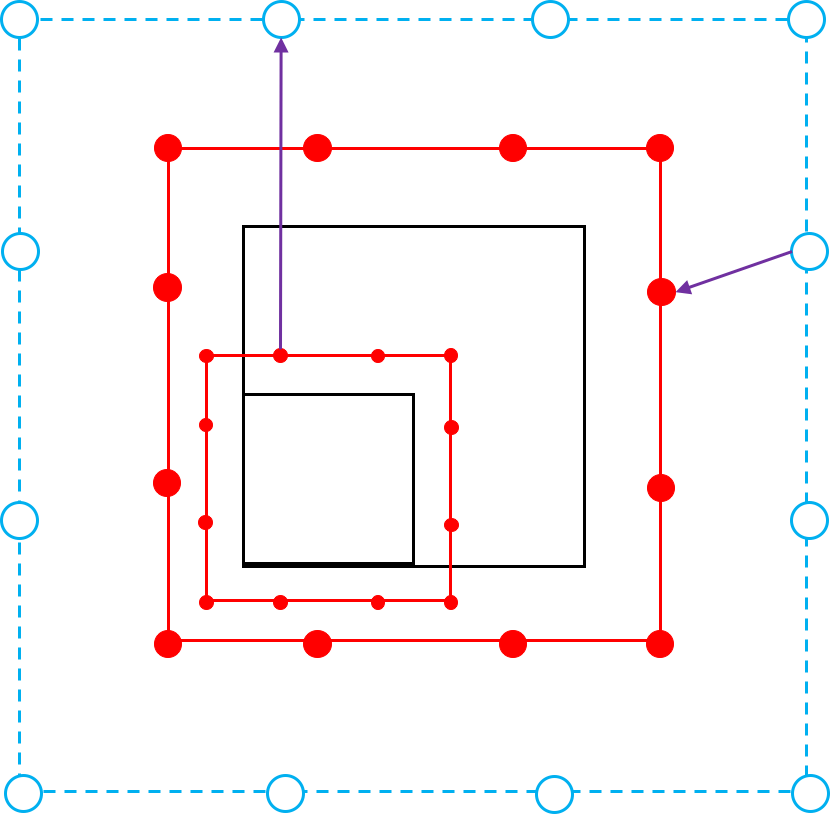
\includegraphics[width=0.4\textwidth]{introduction/kifmm_m2m.png}}
    \hfill
  {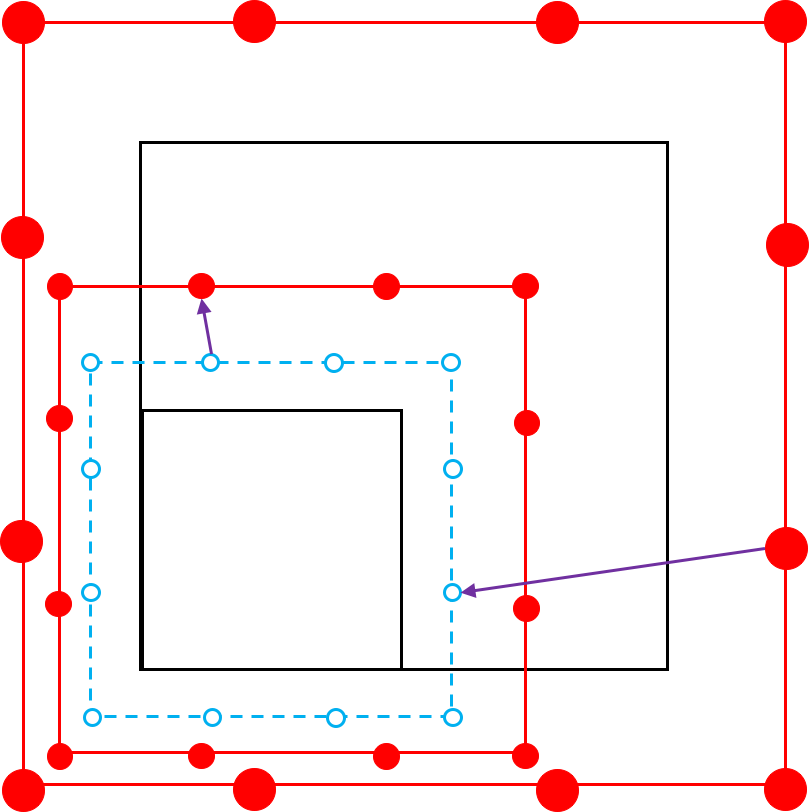
\includegraphics[width=0.4\textwidth]{introduction/kifmm_l2l.png}}
  \vspace{0pt}
  \caption{Cross section of three dimensional cubic surfaces. The (A) \gls{M2M} operation and (B) \gls{L2L} operation. Red solid lines
  denote equivalent surfaces, and blue checked lines denote check surfaces.
  The black solid line defines the box $B$. This figure is adapted directly from \cite{Ying:2004:JCP}.}
  \label{fig:1_2_m2m_l2l}
\end{figure}

The \gls{M2M}, \gls{L2L} and \gls{M2L} operations are illustrated using cubic surfaces in figure (\ref{fig:1_2_m2m_l2l})
The reason for using cubic check and equivalent surfaces are for ease of integration
in the case where the discretisation points chosen are from a regular Cartesian
grid.

\begin{figure}[!h]
    \centering
    {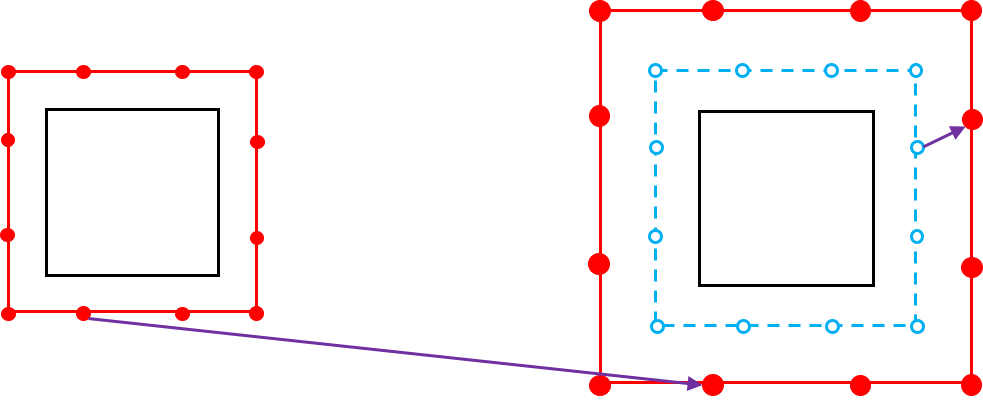
\includegraphics[width=\textwidth]{introduction/kifmm_m2l.png}}
    \caption{Cross section of three dimensional cubic surfaces for the \gls{M2L} operation.
    Red solid lines denote equivalent surfaces, and blue checked lines denote check surfaces.
    The black solid line defines the box $B$.}
  \label{fig:1_2_m2l}
\end{figure}

In principle, it is now possible to replace the kernel function expansions with
the appropriate solutions of the integral equations (\ref{eq:1_2_p2m}),
(\ref{eq:1_2_m2m}), (\ref{eq:1_2_m2l}) and (\ref{eq:1_2_l2l}). However all of
the above equations are ill-conditioned, as they are ill-posed and in general infinite
dimensional problems, and therefore require appropriate regularisation in order to solve.
Consider the following general statement of the first-kind Fredholm equation
that each of the above operations requires,

\begin{equation}
K \phi = q
\label{eq:1_2_first_kind_fredholm}
\end{equation}

This expression reflects the fact that in practical implementations these continuous
integrals are discretised as matrix-vector products. Here $K$ refers to a
`kernel matrix' or operator matrix, which can be found via numerical quadrature, $\phi$ is a vector
of equivalent density to be found, and $q$ is a known vector containing the check
potential. The specifics of the surfaces used in PyExaFMM is discussed in
greater detail in Chapter \ref{chpt:2_strategy_for_practical_implementation},
Section \ref{sec:2_3_operator_caching}. One can use Tikhonov regularisation to
write the solution,

\begin{equation}
\phi = (\alpha I + K^*K)^{-1}q
\label{eq:1_2_tikhonov}
\end{equation}

where $\alpha$ is an appropriate regularisation parameter, and $I$ is the identity
matrix. This equation, a second-kind Fredholm equation, can be solved in numerous
ways. The authors of \cite{Ying:2004:JCP} make use of a Nyström method, and indicate
the possibility of using either Galerkin or Collocation methods. For ease of
implementation, a simpler approach is to instead approximate the solution using a pseudoinverse
estimated from a Singular Value Decomposition, or \textbf{\gls{SVD}}. This
approach is adapted from current C++ implementations of the \gls{KIFMM}, ExaFMM-t,
as well as PVFMM \cite{Malhotra:2015:CCP,exafmm}.

Consider the SVD of a matrix $A$, with $m$ rows and $n$ columns,

\begin{equation}
    A = U \Sigma V^*
\end{equation}

where as usual $U$ is the left singular matrix, $V$ is the right singular matrix
and $\Sigma$ is a diagonal matrix whose elements are the singular values of $A$.
We can write an approximate pseudoinverse of $A$ as \cite{Trefethen:1997:SIAM},

\begin{equation}
    A^\dagger = V \Sigma^\dagger U^*
    \label{eq:1_2_pseudo_inverse}
\end{equation}

here, $A^\dagger$ has $n$ rows and $m$ columns, and $\Sigma^\dagger$ is formed
by taking the reciprocal of all the diagonal elements. Furthermore, to ensure
numerical stability for this reciprocal calculation, one can choose to filter
out components of $V$ and $U^*$ if their singular values smaller than a specified
tolerance. \gls{PyExaFMM} uses this approach to find the pseudoinverse of the
diagonal matrix of singular values $\Sigma$, calculating the pseudoinverse of
the kernel matrix using (\ref{eq:1_2_pseudo_inverse}). The justification of the choices for the regularisation parameter
$\alpha$ and the tolerance for the pseudoinverse are discussed in detail in
Chapter \ref{chpt:2_strategy_for_practical_implementation}, Section \ref{sec:2_3_operator_caching}. In terms of the asymptotic complexity of the \gls{SVD},
as the singular values/vectors are iterated through once in a straightforward
manner to find the pseudoinverse, the complexity of this operation is at most $O(N)$,
where $N$ is the number of singlar values of $A$.

The \gls{KIFMM} algorithm shares almost all of its algorithmic steps with the analytic \gls{FMM}, the
main novelties are the least-squares solves (\ref{eq:1_2_tikhonov}) to compute
the required expansions of each box at each step of the algorithm. In turn
these solves require the computation of the check and equivalent surfaces involved,
as well as the numerical quadrature over the equivalent/source densities to compute
the required check potentials. However, the the matrix to be inverted
in the \gls{M2M} operation as well as the \gls{L2L} operation are very similar, which can
be seen from figure (\ref{fig:1_2_m2m_l2l}). In fact, if
the upward \gls{check-surface} is chosen to coincide with the downward
\gls{equivalent-surface}, and the upward \gls{equivalent-surface} is chosen to
coincide with the downward \gls{check-surface}, the matrix to be inverted for the M2M
operation is the transpose of the matrix to be inverted for the \gls{L2L} operation,
except for a scaling factor dependent on the level of the Octree the surfaces
are created in. This scaling factor is easy to identify, and for the model problem of
three dimensional electrostatics with a Laplace kernel, the scaling factor between
kernel matrices evaluated at two adjacent Octree levels, $l$, is $K^{l+1} = 2K^l$.
Similarly, the required matrix inverse for the \gls{L2L} and \gls{M2L} operations exactly coincide
except for a scaling factor. Therefore, practical implementations
need to compute at most one matrix inversion which can be cached. This can then
be scaled and applied as required at each step of the algorithm. Furthermore,
for the Laplace kernel specifically, the scaling factors are present on both sides
of the equations (\ref{eq:1_2_m2m}) and (\ref{eq:1_2_l2l}), cancelling each other out.
This means that the \gls{M2M} and \gls{L2L} operations can also be calculated between just one
parent box and its respective child boxes, and cached for later use.

Considering the asymptotic complexity of the inverse, its calculation is bound
by a term proportional to the number of singular values of the kernel
matrix, which in turn is dependent on the number of quadrature points chosen for
the check and equivalent surfaces. Therefore as long as this number of quadrature
points is kept small, the pseudoinverse does not effect the asymptotic complexity
of the \gls{KIFMM}. The remainder of the \gls{M2M}, \gls{M2L} and \gls{L2L} operations are bound by
the complexity of computing a matrix vector product between the calculated inverse
matrix and the check potentials, which is resultantly also not impactful on the
algorithm's asymptotic complexity as long as the requirement on the number of
quadrature points is satisfied. As the other algorithmic analysis from
Section \ref{sec:1_1_fmm_overview} remains the same, we can see approximately how
the $O(N)$ complexity is maintained for the \gls{KIFMM}.

\subsection{Summary}

The different approach of the \gls{KIFMM} leads to some different implementation
challenges in comparison to the \gls{FMM}. The key difficulty arises from the
instability in computing the matrix inverse of the kernel matrix between the
check and equivalent matrices. As mentioned, choices for the
regularisation parameter $\alpha$ as well as the tolerance for singular values
taken in the pseudoinverse are discussed with this in mind in Chapter \ref{chpt:2_strategy_for_practical_implementation}, Section
\ref{sec:2_3_operator_caching}.

The ability to cache the \gls{M2M} and \gls{L2L} operators, after calculation for a single
parent box and its respective child boxes, leaves the main bottleneck to
pre-computing all the required operators as the matrix-vector products required
to compute the \gls{M2L} operators. The original authors of the \gls{KIFMM}
accelerate the calculation of the \gls{M2L} operation using a Fast Fourier Transform,
or \textbf{\gls{FFT}} \cite{Ying:2004:JCP}. To see why this can be done, consider
the surfaces describing the \gls{M2L} operation illustrated in figure (\ref{fig:1_2_m2l}),
if the downward \gls{check-surface} of the target box, and the upward
\gls{equivalent-surface} are chosen to be equivalent and lie on a regular Cartesian
grid, then the component of the \gls{M2L} operation that evaluates the action of a
kernel function between these two surfaces can be considered as a convolution
between the kernel function and the equivalent density. Mathematically, if the
kernel function $K(x, y)$ depends only the difference between $x$ and $y$ as it
does for these choices of surfaces for the \gls{M2L} operation, the left hand side of
(\ref{eq:1_2_m2l}) goes to,

\begin{equation}
    \int_{\mathbf{y}^{A,u}} K(\mathbf{x} - \mathbf{y})\phi^{A, u} d\mathbf{y} = q^{B, d}\> \> \text{for any} \> \> \mathbf{x} \in \mathbf{x}^{B, d}
\end{equation}

Padding the empty nodes with zeros allows us to apply the Fourier convolution theorem,
and solve for equivalent density as,

\begin{flalign}
    \phi^{A, u}(\mathbf{y}) = \mathcal{F}^{-1} \left [ \frac{\mathcal{F}(q^{B, d}(\mathbf{x}))}{\mathcal{F}(K(\mathbf{x}))} \right]
\end{flalign}

The currently available major \gls{KIFMM} implementations use this to accelerate the calculation of the
\gls{M2L} operator including ExaFMM-T and PVFMM \cite{Malhotra:2015:CCP, exafmm}.  Though
reasoned in more detail in Chapter \ref{chpt:2_strategy_for_practical_implementation}, Section \ref{sec:2_3_operator_caching}, we state for
the present that the expansion order $p$ is by definition proportional to the
number of quadrature points used to discretise the surface of the check and
equivalent surfaces. Specifically, PyeExaFMM follows the example of ExaFMM-T and
PVFMM, taking the relationship between $p$ and number of quadrature points, $n_q$,
to be,

\begin{equation}
    n_q = 6(p-1)^2 + 2
\end{equation}

Meaning that each surface has $O(p^2)$ points, and therefore the \gls{M2L} operation
(\ref{eq:1_2_m2l}) is of $O(p^4)$ between a given target box and source box.
This FFT based method to find equivalent densities, accelerates the \gls{M2L} calculation between a given target box
and a given source box to $O(p^3 \log(p))$. In PyExaFMM we use an alternative
acceleration scheme, based on low rank SVD approximations, discussed further in
Chapter \ref{chpt:2_strategy_for_practical_implementation}, Section \ref{sec:2_4_svd_compression}. Therefore we defer to the
literature for further details on FFT based acceleration methods \cite{Malhotra:2015:CCP}.

The \gls{KIFMM} presents many of the same opportunities for parallel implementation
as the \gls{FMM}. In terms of \gls{task-level-parallelism}, PyExaFMM implements
parallel processing, via Python's native multiprocessing tools, for the calculation
of the \gls{M2L} operations. As these calculations involve dense matrix-vector products,
they are also ideal candidates to be transferred
to a \gls{GPU} for rapid parallel evaluation in the future. PVFMM implements
\gls{task-level-parallelism} for the calculation of the M2M, L2L, and M2L
operators with \textbf{\gls{MPI}} as well as an interface with \gls{CUDA} for
processing the dense matrix-vector products. ExaFMM-T makes use of
\textbf{\gls{OpenMP}} for a similar purpose.

In summary, the key benefits of the \gls{KIFMM} lie in the ability to write
an implementation that is compatible with a wide class of kernel functions,
without evaluating the expansion coefficients. This greatly reduces the complexity
of the software design to support multiple applications of the FMM across
different problem settings. Furthermore, the formulation of the key FMM operations
as dense matrix-vector products makes it easy to map portions of the \gls{KIFMM}
to dedicated parallel hardware such as \gls{GPU}s. The fact that KIFMM logic
is not dependent on the form of the kernel function expansion, and just on kernel
function evaluations,  makes it trivial to separate the concerns of a software
implementation, and write optimisation libraries for the KIFMM independently of
the main loop (fig. \ref{fig:1_1_main_loop}) itself. The impact on software design
and architecture is signficant, and is explored further in Chapter \ref{chpt:2_strategy_for_practical_implementation} Section
\ref{sec:2_5_software_design}. This design is the key benefit of \gls{PyExaFMM}
in comparison to existing \gls{KIFMM} implementations, as \gls{PyExaFMM} is already
sacrificing a degree of performance via the choice of implementation language,
we are able to implement some effective software engineering principles
to ease the burden on a user in terms of debugging and expanding upon \gls{PyExaFMM}.
